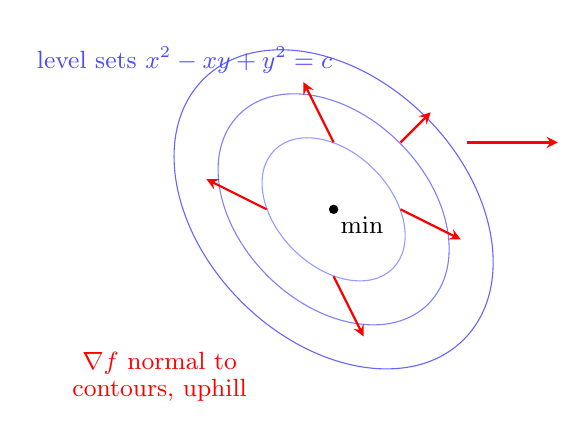
\begin{tikzpicture}[scale=0.85,>=stealth]
% f = x^2 - xy + y^2 level sets are ellipses rotated 45deg: f = (x^2+y^2)/2 in rotated coords ~ radius sqrt(2c/3) and sqrt(2c)
\begin{scope}[rotate=45]
\draw[blue!40] (0,0) ellipse (0.85 and 1.25);
\draw[blue!50] (0,0) ellipse (1.4 and 2.0);
\draw[blue!60] (0,0) ellipse (1.95 and 2.75);
\node[blue!70] at (0,3.15) {\small level sets $x^2-xy+y^2=c$};
\end{scope}
% arrows: (1,0)->(2,-1), (0,1)->(-1,2), (1,1)->(1,1), (-1,0)->(-2,1), (0,-1)->(1,-2), scaled 0.45
\draw[->,red,thick] (1,0)--(1.9,-0.45);
\draw[->,red,thick] (0,1)--(-0.45,1.9);
\draw[->,red,thick] (1,1)--(1.45,1.45);
\draw[->,red,thick] (-1,0)--(-1.9,0.45);
\draw[->,red,thick] (0,-1)--(0.45,-1.9);
\draw[->,red,thick] (2,1)--(3.35,1.0);
\fill (0,0) circle (2pt) node[below right=-1pt]{\small min};
\node[red] at (-2.6,-2.3) {\small $\nabla f$ normal to};
\node[red] at (-2.6,-2.7) {\small contours, uphill};
\end{tikzpicture}
